\chapter{User Guide}

\label{ch:guide}

\section{Feature vectors}

As the first step in re-identification process, we need to extract useful information
from each detection we are tasked to identify. This process serves multiple purposes.

If we encode every useful information from the image of the detection, we can discard
the crop itself after generating the feature vector. This may significantly decrease
the amount of space we need to reserve to store the information regarding the detections.
Although, the ratio of how much memory we can save by this process heavily rely on
the fact how the feature vector is generated (and how big the final vector is).
Furthermore, if it is possible to generate the feature vectors on-line we can entirely
skip the step of storing the detections in the database and decrease the memory
requirements even further.

Other significant advantage of this process is the anonymization. Unless the generated
feature vector is reversible, we can entirely anonymize the images of potentially
sensitive images.

Nevertheless, the goal is to not supply the re-identification algorithm with the original
crop but rather corresponding feature vector. Therefor, we also need to convey
as much information in regards to identification into the feature vector as possible.
Generally, this means that we want detections to lead to the feature vectors that are
close (in terms of suitable distance, like euklidean distance) to the feature vectors
from other detections from the same identity (although details depend on the 
used re-identification algorithm).

\subsection{Running the Algorithm}
\label{sec:running_annotator}

All the algorithms for creating the feature vectors are implemented in the file
\texttt{ReID\/annotator.py}. The annotation process itself can be started independently
of other parts of the framework, as long as the annotated detections are already
inserted into the database.

Annotation can be started by following command:
\begin{verbatim}
    $ python -m ReID.annotator
\end{verbatim}
However, such command needs to be followed by various options and then by selected
algorithm for annotation (and then options specific for given algorithm). An example of 
complete command for annotation is:
\begin{verbatim}
    $ python -m ReID.annotator --log DEBUG -c 468 --class person\
      -p 1000 -j 8 resnet-prepare --shape 48 48
\end{verbatim}

In this case global options are (\verb+--log+, \verb+-c+ and \verb+--class+). They are 
followed by selection of specific annotating algorithm (\verb+resnet-prepare+). At 
the end of the command are options for that specific algorithm (\verb+--shape+).

% \begin{figure}
%     \begin{verbatim}
% usage: annotator.py [--log {DEBUG,INFO,WARNING,ERROR,CRITICAL}]
%                     [-h] -c CAMERA[--class CLASS] [-p PAGE_SIZE]
%                     [-j JOBS] [-f] {simple-hue-histogram,
%                     cropped-hue-histogram,gauss-hue-histogram,
%                     resnet-prepare,mobilenet-prepare}
%                     ...

% positional arguments:
%   {simple-hue-histogram,cropped-hue-histogram,gauss-hue-histogram,resnet-prepare,mobilenet-prepare}
%                         Annotator to use for the annotation
%   annotator_arguments   Additional arguments for chosen annotator

% optional arguments:
%   -h, --help            show this help message and exit
%   --log {DEBUG,INFO,WARNING,ERROR,CRITICAL}
%                         Threshold for logger level
%   -c CAMERA, --camera CAMERA
%                         ID of camera to annotate
%   --class CLASS         Class to annotate (e.g. PERSON), if omitted all
%                         classes are annotated
%   -p PAGE_SIZE, --page-size PAGE_SIZE
%                         Number of detection requested from database at one
%                         time. Setting this to low number decreases local RAM
%                         usage but increases the number of database requests.
%                         To disable paging altogether, set this to 0
%   -j JOBS, --jobs JOBS  Number of jobs (threads) to use
%   -f, --force-update    Recompute descriptors even if they are already present
%     \end{verbatim}
%     \caption{Help message for annotator algorithm}
%     \label{fig:annotator_help}
% \end{figure}

Most of the global options are explained in the help message (obtained by using
\verb+--help+ flag) as you can see in Figure \ref{fig:annotator_help}. In standard
mode if the algorithm already finds the detections are already annotated with this
specific options if will report this error and will not run. This behavior can be
overridden by the \verb+--force-update+ option.

Other more complicated option is \verb+--page-size+. This parameter sets how many
records will be requested from the database at once. Setting this to very high number
(or disabling completely) may result in problems with unsufficient memory, as the 
algorithm needs to store at the same time that many records (most notably, images of 
detections). On the other hand, setting this to very low number will result in
significantly slower annotation as it increases number of database requests needed.
This also affect the progress bar showing number of annotated detections. The progress
bar updates after the whole batch is annotated, this means that for high number the
progress bar is updated in large intervals and for low numbers the progress bar works
far smoother.

\section{Color-based feature vectors}

As one of the more basic approachas for generation of feature vector we extract colors
from the images of detections. The idea here is that the different detection of the same
person should have roughly look same in terms of colors. Of course, if we focus on
re-identification within a single camera, spatial information will still be far more
important than such feature vector. Howerver, we can reasonably except that the colors
of the detections will remain the same even across several cameras, especially if the
cameras are will capture the object from roughly the same angle.

In order to mitigate the effect of illumination and shadows, we firstly convert the
detection images into the HSV encoding and then extract the HUE part of the encoding.
For each detection we then proceed the construct a histogram of HUE. Such histograms
should reasonably well represent the color distribution, hence the image of the same
person should be resonably similar. We will further investigate these claims in the 
Chapter \ref{ch:evaluation}.

In order to annotate the detection with such simple histograms, one can use:
\begin{verbatim}
    $ python -m ReID.annotator -c <camera_id>\
      simple-hue-histogram --bins 50
\end{verbatim}

Of course, we can use other global flags as described in Section 
\ref{sec:running_annotator}. Apart from them this annotator offers another specific
flag \verb+--bins+. This parameter describes the number of bins for the histogram.

The program will fetch all the corresponding detections, computes the histogram
of given parameters and stores them in database in form of raw numpy array
(\cite{numpy}). The images may be of varying sizes and dimensions (e.g. images
from vidoes in higer dimesnsion may have twice as many pixels as images from video
of lower resolution, making the histogram significantly different). To counter this
problem we normalize the histogram, so sizes of bins represent ratio of given color
within the image rather than absolute number of pixels with given color.

\subsection{Background elimination}

One of the problem with such basic approach is that the large part of the detection
image consists of the background. This may significantly shift general color composition
of the image and thus change the historgam.

One can notice, that the actual object is usually in the middle of the detection and the
corners are in vast majority of the cases filled with the background. Therefor, we
present few simple techniques that focuses on the middle of the image, as such focus
should capture more of the object and less of the background, making the resulting
histogram more representative.

\subsubsection{Cropped image}

The simplies possible solution for this problem is to crop the image even further 
and taking into consideration only the middle part of the image. This aproach we can
test via running the following:

\begin{verbatim}
    $ python -m ReID.annotator -c <camera_id> \
      cropped-hue-histogram\
      -b <bins> -x <from_x> <to_x> -y <from_y> <to_y>
\end{verbatim}

The \verb+--bins+ (or \verb+-b+) command works the same as in case of simple histograms.
New options \verb+-x+ and \verb+-y+ allows us to specify the crop we want to consider
for histogram generation. For each of these flags we need to specify lower and upper
boundary of $x$-axis (horizontal) and $y$-axis (vertical) axis. The boundaries are
relative to the width and height of the detection image. Thus, for example setting $x$ 
and $y$ boundaries to 0 and 1 will result in the same result as not using cropped
histogram at all. More useful example is to setting the boundaries to $0.25$ and $0.75$,
which will extract the middle part of the image. However, one may consider for $y$ axis
setting boundaries to capture part of the image closer to the top (as we usually
capture people, and this way we may evaluate torso, arguably the most telling part).
As we consider coordinate 0,0 to be top-left, to capture part of the image closer
to the top, one should set \verb+-y+ paremater for example to $0.15\,0.65$.

\subsubsection{Gaussian weighting}

We offer one more ``smoother'' approach to mitigate the influence of the background.
Rather than just consider the pixels in the middle of the image and discard the rest,
we increase the weights of the pixels closer to the middle and decrease the weight
of pixel near borders.

Most straight-forward weighting function that fulfills required properties (positivity
over whole domain, single maximum and decreasing everywhere in direction away from the
maximum) is Gaussian function. Therefore, we present another algorithm utilizing this
exact approach. Such algorithm can be run as follows:

\begin{verbatim}
    $ python -m ReID.annotator -c <camera_id> \\
      --bins <bins> -x <x> -y <y> -s <scale>
\end{verbatim}

Parameter \verb+--bins+ works same as in previous algorithms. Parameters \verb+-x+ and
\verb+-y+ sets the coordinate of the maximum weight. These are relative to the dimensions
of the crop, thus setting both to 0.5 will cause to maximum to be in the middle of the
crop, however one may wish to set the \verb+-y+ to for example 0.3 to set maximum to
upper part of the image (as discussed in previous section). Finally the \verb+-s+
parameter sets the spread of corresponding Gaussian function (again scaled to the 
relative dimensions of the image). If we set this parameter
to very small numbers, few pixels close to the coordinate with maximal importance will
essentially define the resulting histogram, while coordinates near the border will
have almost no effect. Higher the value of this parameter the weights of the pixels are
more balanced, setting this to very high number will have the same effect as not using
the weight at all (as all the pixels will have very similar weight).

The weight of a pixel at coordinates $x$ and $y$ can be described as:\footnote{note that 
in actual implementation we use probability distribution function (using scikit -- 
\cite{scipy}), so the computed values differ by a coefficient, this difference however 
does not influence the resulting histogram as we normalize it}
$$w(x,y) = \exp\left(\frac{-1}{2\sigma^2} \left[\left(\frac{x}{x_m}-x_o\right)^2 - \left(\frac{y}{y_m}-y_o\right)^2 \right]\right)$$
In this equation the $x_o$ and $y_o$ correspond to the coordinates with maximal
weight (i.e. values set by \verb+-x+ and \verb+-y+ respectivelty) and $x_m$ and $y_m$
refer to maximal boundaries (i.e. width and height of an image).

\section{Annotation tool}

Just like in any other case of a machine learning algorithm, we needed annotated data even in our case. As the videos used for development and testing the re-identification algorithm was several minutes long, there were thousands of frames and tens of thousands
of detections for annotation.

In order to make the annotation as easy as possible, we present an annotation tool that we used during the development of our algorithms. While the annotation was the primary task, we can use the tool for the exploration of results of both, various 
\emph{reidentifictaiton} algorithm and also algorithms that output just 
\emph{trajectories}.

\subsection{Tool options}

The annotation tool is, as other parts of this work, designed as a module of the whole
framework for in-video identification and to be used as a library. However, as the
nature of the tool requires, we also implemented a standard command-line interface.
The tool can be invoked (after installation of all dependencies) as follows:

\begin{verbatim}
$ python3 -m ReID.explore    
\end{verbatim}

A list of parameters required for the annotation tool to run can be obtained by running
the took with \texttt{\-\-help} flag. Description of various options can be seen in
figure \ref{fig:annotation_tool_help}

% \begin{figure}
%     \begin{verbatim}
% usage: explore.py [-h] [--log {DEBUG,INFO,WARNING,ERROR,CRITICAL}]
%                   -c CAMERA_IDS [CAMERA_IDS ...] [-f FILE]
%                   [-t TRAJECTORY_MODEL_ID] [-i IDENTITY_MODEL_ID]
%                   [-p] [--fullscreen]

% optional arguments:
%   -h, --help            show this help message and exit
%   --log {DEBUG,INFO,WARNING,ERROR,CRITICAL}
%                         Threshold for logger level
%   -c CAMERA_IDS [CAMERA_IDS ...], --camera_ids CAMERA_IDS
%                         [CAMERA_IDS ...] ID of camera(s) to
%                         explore
%   -f FILE, --file FILE  Name of the file to load trajectory model
%                         from
%   -t TRAJECTORY_MODEL_ID, --trajectory TRAJECTORY_MODEL_ID
%                         ID of base trajectory model
%   -i IDENTITY_MODEL_ID, --identity IDENTITY_MODEL_ID
%                         ID of base identity model
%   -p, --preload         Preload all detection in initialization
%   --fullscreen, --fs    Run in fullscreen mode
%   -s SCALE, --scale SCALE
%                         Scale the screen of the camera(s) by given
%                         factor
%   -k CLASS, --class CLASS
%                         If specified, show only detections of
%                         given class
%   --start START_TIME    Query only frames from this timestamp onwards
%                         (relative to the first frame of this camera)
%   --end END_TIME        Query only frames up to this timestamp (relative to
%                         the first frame of this camera)


%     \end{verbatim}
%     \caption{Annotation tool help output}
%     \label{fig:annotation_tool_help}
% \end{figure}

As we already stated, the annotation tool is capable of handling both -- results of re-identification and the results of trajectory generation. From the command line we
make this distinction by either specifying the \emph{trajectory model} id (the
\texttt{\-\-trajectory} option) or the \emph{identity model} id (the
\texttt{\-\-identity} option. Either way, the selected IDs should correspond to the
ID of the model in database (form the \texttt{traj\_model} resp. 
\texttt{identity\_model}). Shown detections will then be displayed in the context
of the selected model.

Furthermore, instead of selecting direct trajectories or identifications from the
database, we can load these from the file that was generated by the previous run of
annotation tool. This may be useful if we do not want to save the annotated data
into the database but want to save the intermediate results (this way we can save
time by as these files may be stored locally, rather than uploaded on remote
server).

We select the input stream via the \texttt{\-\-camera\_ids} option. These IDs should
correspond to the IDs of cameras in the \texttt{camera} table. If we browse the
results of \emph{trajectory} detection, we may naturally select just one camera
as an input. On the other hand, if we are exploring the results of
\emph{re-identification}, we should list all the cameras that were presented
for the generation of the re-identification. The program will then find and select
appropriate \emph{camera setup} from the database.

In standard behavior, the detections are loaded on-demand. This means that the detections
are queried just after displaying their frame (unless given frame was already loaded).
As a result, the user may experience a short lag whenever he switches to a different frame.
In order to eliminate or at least minimize this delay, we implement the
\texttt{\-\-preload} option. With this flag on, all the detections are loaded on the
lunch of the tool. This will significantly prolong the start-up of the application; on the other hand, the whole experience of using the tool is smoother.

If we attempt to annotate data that comes from the source that is in higher resolution
than our current display, whole annotation tool does not fit into screen. For this case
we also implemented scaling of the display, so we can make the source detection smaller,
effectivelly fitting in our screen. Scaling option can be turned on by the
\texttt{\-\-scale} option, followed by the factor we want to scale (i.e. if we want the
source input to seem twice as small we input factor 0.5). Via the same option we can
make the detection bigger if we wish so.

If we do not want to query all the frames, we can use options \verb+--start+ and
\verb+--end+. These options will make the application to query only frames and detection
within given offset from the first frame of the stream. For example \verb+--end 00:01:00+
will cause that only frames from the first minute of the video will be loaded.
Combination of options \verb+--start 00:01:00+ and \verb+--end 00:02:00+ will load
frames from the second minute of the video. This is especially useful when used with
the \verb+--preload+ options. As normally are detections loaded on-demand there is very
little speed-up if we use \verb+--start+ and \verb+--end+ by themselves. However, when
using \verb+--preload+ all the detections are loaded at, startup; giving time interval
to load detection from can dramatically decrease number of detections loaded and thus
significantly speed-up the start up of the application.

\subsection{User Interface}

After launching the application, the detections from the first frame of the corresponding
camera (or cameras) are displayed. Example of such screen is shown in figure
\ref{fig:annotation_tool_screenshot}.

% \begin{figure}
%     \centering
%     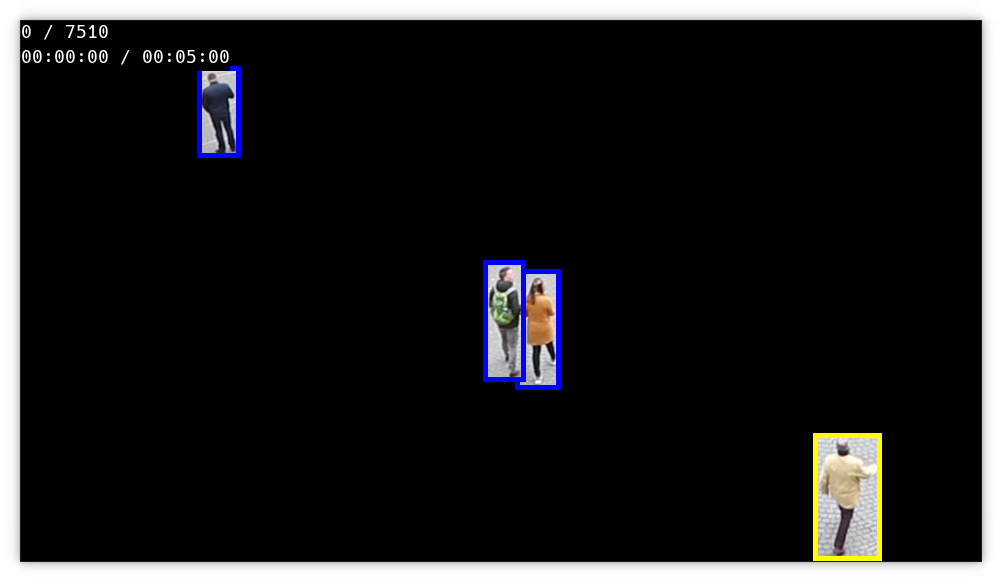
\includegraphics[width=\textwidth]{../img/annotation_tool_screenshot.png}
%     \caption{Example of the first frame of the annotation tool}
%     \label{fig:annotation_tool_screenshot}
% \end{figure}

After launching the application, we can see highlighted detections from
the first frame of the video on the screen.
Only detections are shown, not the whole video, in this way, we do not need access
to the original video (just data already presented in the database). In the top left corner
of the screen, we can see the sequence number of the frame (this is not the frame ID
in the corresponding database, just a sequence number within the respective stream). Alongside
the sequence number is displayed the timestamp of the displayed frame.

We can browse the video by right and left arrows, skipping one frame forward and
backward, respectively. Each time we skip on a different frame, the detections from
the new frame are rendered and highlighted. However, the old detections are left
on the screen for better referencing the previous screen. The user can refresh the display
and hide all detections apart from detections from the current frame by hitting \verb+c+.
For other commands allowing to browse the stream refer to table
\ref{tab:annotation_basic_commands}

By clicking on the detection with a mouse button user can select given detection (or rather trajectory/identity of the corresponding detection). One identity can be selected
by the left mouse button and one other by the right mouse button. Selected identities can then be unified via \verb+unify+ command. One can also select a detection with the
middle mouse button. Unlike selection with the left and right mouse button, the application
allows for multiple identities to be selected with the middle mouse button. Such selection
does not serve the purpose of annotation directly (does not work with \verb+unify+ command.
However, it marks the given identity as already processed. Annotators can then use the Up and Down key for scrolling more efficiently. Refer to table 
\ref{tab:annotation_basic_commands} for further explanation of Up and Down commands.

\begin{table}
    \centering
    \begin{tabularx}{\textwidth}{l|X}
         \textbf{Key} & \textbf{Command} \\ \hline
         Right arrow & Skip one frame forward \\ \hline
         Left arrow & Skip one frame back \\ \hline
         Up arrow & Skip frames until the one with detection that is not selected
         via left, right or middle mouse button or to the end of the stream \\ \hline
         Down arrow & Skip frames backwards until the one with detection that is not selected via left, right or middle mouse button or to the first frame \\ \hline
         Page up & Skip 10 frames forward \\ \hline
         Page down & Skip 10 frames back \\ \hline
         Home & Skip to the first frame \\ \hline
         End & Skip to the last frame
    \end{tabularx}
    \caption{Basic controls of annnotation tool}
    \label{tab:annotation_basic_commands}
\end{table}

Each selection is associated with a different highlight color for given detections.
For explanation of given colors, please refer to table \ref{tab:annotation_highlight}

\begin{table}[]
    \centering
    \begin{tabularx}{\textwidth}{l|X}
         \textbf{Color} & \textbf{Explanation} \\ \hline
         Blue & Unselected detections that are assigned into an identity \\ \hline
         Yellow & Detections that are present on the frame but are not part of any
         identity for loaded model \\ \hline
         Red & Detections/identities selected via left mouse button \\ \hline
         Green & Detections/identities selected via right mouse button \\ \hline
         Cyan & Detections/identities highlighted via middle mouse buttn \\
    \end{tabularx}
    \caption{Highlight color of detections}
    \label{tab:annotation_highlight}
\end{table}

\subsection{Fast exploration of interesting detections}

\label{subsec:exploration}

Aside from the standard controlling mechanism, we offer additional features especially
useful for exploring incorrectly identified and annotated identities. We allow
for a loading list of pairs of identities during the exploration of the results. These
identities can be quickly searched through. By this method, we an, for example, efficiently fix the incorrectly annotated data in the golden dataset if we obtain a list of ``suspicious'' identities (for example list of identities that our re-identification algorithm classified differently than are classified in the golden dataset).

The list itself should state two identities ID (corresponding to the IDs in the
database) on each line, separated by space. The lines that start with the hash (\verb+#+) are considered as comments and not processed. Once the pairs are loaded
from the file with \verb+load_pairs+ command, given pairs can be processed via other
commands, refer to section \ref{sec:commands} for a complete list of commands.

\subsection{Commands}
\label{sec:commands}

By typing colon (\verb+:+) the user enters the command mode. Then the user can type
a command which will be displayed at the lower part of the screen. Commands are confirmed
by hitting enter and canceled via Escape. List of available command is:

\begin{itemize}
    \item \verb+unify+ (or hitting \verb+u+ in standard mode) -- merge all detections
    from identity selected by right mouse button into identity selected by left mouse 
    button
    \item \verb+hide+ (or hitting \verb+h+ in standard mode) -- hide the identity
    currently selected with the left mouse button (detections from given identity
    will be treated as if they would not be part of any identity at all, i.e.
    highlighted in yellow if all the detections are visible, or not displayed at all
    if user hid them via \verb+all+ command).
    \item \verb+all+ (or hitting \verb+a+ in standard mode) -- stops showing detections
    that are not part of any identity. If these detections are already hidden, start
    showing them instead
    \item \verb+quit+ (or hitting \verb+q+ or \verb+Esc+ in standard mode) -- terminates
    the application
    \item \verb+left+ (or hitting \verb+l+ in standard mode) -- find and skip to the
    first frame where is detection selected by left mouse button. Frames are searched
    starting from the current frame onwards (previsou frames are not searched at all)
    \item \verb+right+ (or hitting \verb+r+ in standard mode) -- works same as the 
    \verb+left+ command, except it searches for detections selected with right mouse
    button
    \item \verb+transfer+ (or hitting \verb+t+ in standard mode) -- move the detection
    from the identity selected by right mouse button that is currently displayed from
    its identity into identity selected by left mouse button.
    \item \verb+single_auto+ (or hitting \verb+s+ in standard mode) -- create new
    identity/trajectory and assign currently displayed detection that is part of the
    identity/trajectory selected by right mouse button into it.
    \item \verb+id+ (or hitting \verb+i+ in standard mode) -- start showing IDs of
    detections below the currenly highlighted detections. These correspond to the IDs
    in the \texttt{detection} table.
    \item \verb+memory+ (or hitting \verb+m+ in standard mode) -- repeat the last search 
    for deteciton (invoked with commands
    like \verb+left+, \verb+right+, \verb+find+ or \verb+next+
    \item \verb+postpone+ (or hitting \verb+p+ in standard mode) -- mark last searched 
    pair of identities as not resolved. This pair will appear in form of comment should
    the pairs be saved in this session.
    \item \verb+next+ (or hitting \verb+n+ in standard mode) -- search for next pair
    of identities loaded via \verb+load_pairs+ command. This will automatically skip
    to the first frame with the detection from the first identity. Furthermore, the
    first identity will be selected with left mouse button and the second with the
    right mouse button. Given pair will be marked as processed, meaning that it will
    not appear in the file for subsequent \verb+save_pairs+ command (unless the pair
    is postponed via \verb+postpone+ command).
    \item \verb+clear+ (or hitting \verb+c+ in standard mode) -- refresh the view.
    This will delete all the detections displayed for other frames and leaves only
    the detections from current frame.
    \item \verb+delete+ (or hitting \verb+d+ in standard mode) -- remove identity
    selected by left mouse button from the moden entirely
    \item \verb+save <file_path>+ -- store the current model into a local file
    specificied via \verb+<file_path>+ if given file does not exists
    \item \verb+save! <file_path>+ -- works same as the \verb+save+ command except
    it overrites given file if it exists
    \item \verb+upload <generator_name> <options>+ -- stores current model into the
    database as model with given parameters
    \item \verb+find <detection_id> [(l|r|<detection_id>)]+ -- skips to the frame
    with detection with given \verb+<detection_id>+. If the ID is followed by \verb+l+,
    automatically select the detection via left mouse button, if it is followed by
    \verb+r+ select it via right mouse button. If the ID is followed by second
    \verb+<detection_id>+, select the detection corresponding to the first ID by left
    mouse button, and the detection corresponding to the second ID by right mouse button
    \item \verb+single <detection_id>+ -- create a new identity/trajectory. Assign the
    detection with \verb+<detection_id>+ into it.
    \item \verb+load_pairs <file_path>+ -- load list of pairs of identities (as per subsection \ref{subsec:exploration}). 
    \item \verb+save_pairs <file_path>+ -- save all remaining pairs of identities that were loaded via \verb+load_pairs+ and not processed via \verb+next+ command. The
    pairs are saved to the corresponding \verb+<file_path>+, unless given file already
    exists
    \item \verb+save_pairs! <file_path>+ -- works the same as the \verb+save_pairs+
    command, except it overrides the file \verb+<file_path>+ if it exists
    \item \verb+select_left <identity_id>+ -- select identity \verb+<identity_id>+ 
    as with the left mouse button and
    skip to the first frame with the detection from given identity
    \item \verb+select_right <identity_id>+ -- works the same as \verb+select_left+
    command, except it select given identity with the right mouse button.
\end{itemize}

